% !TeX root = ../main.tex
\section{背景与动机}
\label{sec:background}

\subsection{浮点精度与微缩放格式}
\label{sec:formats}

BF16/FP16 由逐元素的指数与有效数确定动态范围和精度~\cite{burgess2019bfloat16}；微缩放格式则将低位宽元素与共享尺度共同编码（图~\ref{fig:fpformats}）。OCP MXFP8/6/4 采用 32 元素一组的 E8M0 尺度~\cite{ocpmx2023}；NVFP4 使用 16 元素一组的 E4M3 尺度~\cite{nvidia2024nvfp4}；HiF4 使用 64 元素一组的无符号 E6M2 基础尺度，并为每 8、4 个元素分别配置一位微指数~\cite{hifloat4}。元素编码、分组粒度和尺度编码分别决定解包、局部规约与尺度融合的硬件需求。

\begin{figure}[t]
\centering
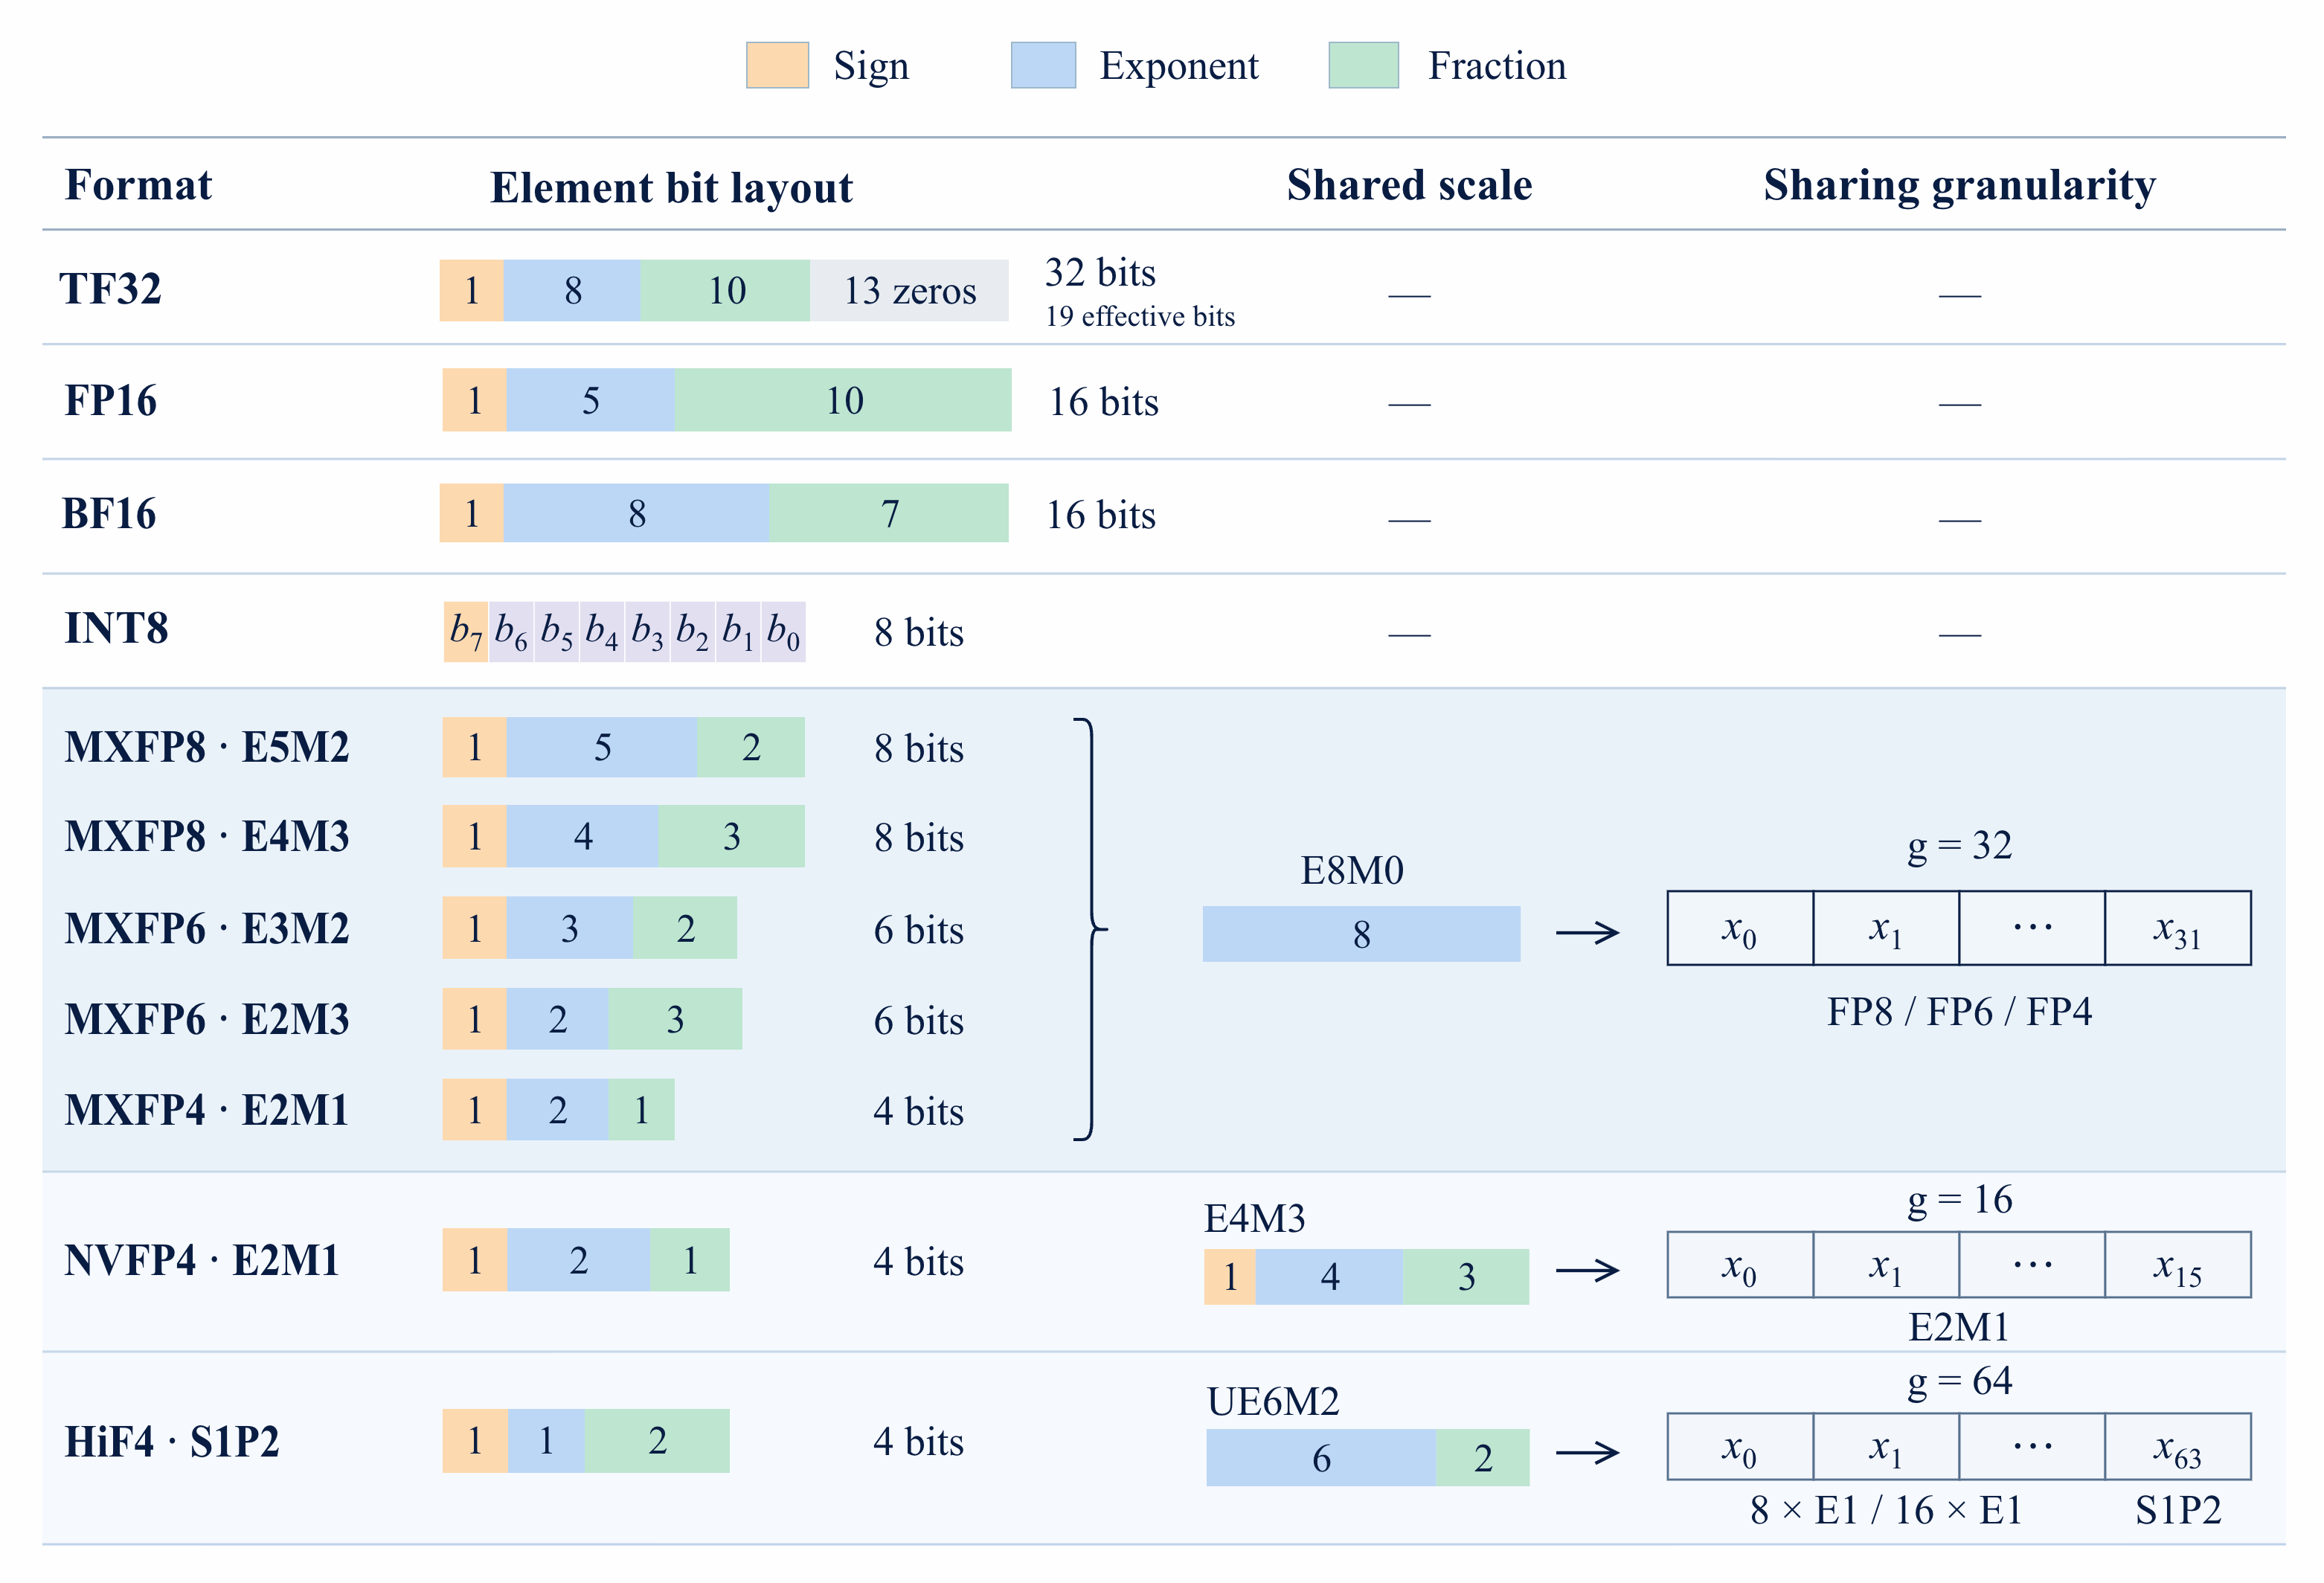
\includegraphics[width=\columnwidth]{fp_format.png}
\caption{元素编码与共享尺度~\cite{ocpmx2023,nvidia2024nvfp4,hifloat4}。字段标注为位宽，$g$ 为缩放组大小。}
\label{fig:fpformats}
\end{figure}


\subsection{张量计算与点积单元}
\label{sec:tensor_organization}

对于矩阵乘累加 $D=C+AB$，$M$、$N$ 是输出维度，$K$ 是归约维度。点积单元先对齐多个乘积并集中归约，再统一规格化和舍入，以共享后端摊薄逐项浮点处理的成本~\cite{lutzFusedFP84Way2024}。本文采用 H 类原生归约长度为 16 的 DP 作为基线，与已有数值建模研究识别的点积累加粒度相对应~\cite{xie2025mmasim}。完整 GEMM 沿归约维拆为多笔请求，单 DP 接收显式 $C$ 并输出 $D$，跨请求部分和保存在其外部。

有无组尺度的格式可用同一局部点积结构描述。依据 OCP 的点积定义，共享尺度可提出组内归约~\cite{ocpmx2023}。将 $L$ 项乘积按缩放组边界划分为 $G=\lceil L/g\rceil$ 组，末组不足部分补零，加入累加输入 $c$ 后，有
\begin{equation}
d=c+\sum_{j=0}^{G-1}X_j^{(A)}X_j^{(B)}
\underbrace{\sum_{i=0}^{g-1}P_{j,i}^{(A)}P_{j,i}^{(B)}}_{q_j}.
\label{eq:blockdot}
\end{equation}
其中，$X_j^{(A)}$、$X_j^{(B)}$ 为两路输入第 $j$ 组的共享尺度，$P_{j,i}^{(A)}$、$P_{j,i}^{(B)}$ 为组内元素的解码值，$q_j$ 为组内点积；HiF4 的局部微指数计入元素解码。对于无组尺度的格式，令 $X_j^{(A)}=X_j^{(B)}=1$，即可得到普通点积累加。

式~\eqref{eq:blockdot} 给出分层共享的算术边界；内部位宽、顺序与舍入仍由具体实现约束。



\subsection{通路复用与设计空间探索}
\label{sec:datapath_sharing}

表~\ref{tab:related_features} 汇总格式与组合能力。MX 列区分完整微缩放支持与仅元素运算支持；本文通过在共享 DP 内增配专用 Group 改变算力配比。

% Entries refer to reported configurations, not hypothetical reconfiguration.
\begin{table*}[t]
\centering
\caption{Supported input formats and datapath features of related arithmetic units.}
\label{tab:related_features}
\begingroup\footnotesize\setlength{\tabcolsep}{3pt}
\def\Y{$\checkmark$}\def\N{$\times$}
\begin{tabular*}{\textwidth}{@{\extracolsep{\fill}}l*{14}{c}@{}}\toprule
& \multicolumn{9}{c}{Native input formats} & \multicolumn{5}{c}{Datapath features} \\
\cmidrule(lr){2-10}\cmidrule(lr){11-15}
Design & TF32 & FP16 & BF16 & FP8 & FP6 & FP4 & INT8 & INT4 & LOG4 & DP & MX & NVFP4 & HiF4 & SR \\\midrule
Ten-Four~\cite{rout2026tenfourv2} & \Y & \Y & \Y & \Y & \N & \N & \Y & \Y & \N & \Y & \Y & \N & \N & \N \\
MPICC~\cite{huangMPICCMultiplePrecisionInterCombined2025} & \N & \N & \N & \Y & \Y & \Y & \N & \Y & \Y & \Y & --- & \N & \N & \Y \\
MXDOTP~\cite{islamoglu2025mxdotp} & \N & \N & \N & \Y & \N & \N & \N & \N & \N & \Y & \Y & \N & \N & --- \\
FPnew~\cite{mach2020fpnew} & \N & \Y & \Y & \Y & \N & \N & \N & \N & \N & \N & \N & \N & \N & \N \\
TransDot~\cite{transdot2026} & \N & \Y & \N & \Y & \N & \Y & \N & \N & \N & \Y & \N & \N & \N & --- \\
\midrule
DP-Puzzle & \Y & \Y & \Y & \Y & \Y & \Y & \Y & \N & \N & \Y & \Y & \Y & \Y & \N \\
\bottomrule\end{tabular*}
\par\smallskip
\parbox{\textwidth}{\raggedright
$\checkmark$: supported; $\times$: absent from the reported configuration; ---: not established by the cited evidence.
DP: native multi-term dot product; MX/NVFP4/HiF4: integrated block-scale handling (MX indicates at least one MX format); SR: stochastic rounding.
FP8/FP4 denote element arithmetic and do not imply scale support. FPnew additionally supports FP32/64; TransDot supports FP32 FMA. MPICC supports heterogeneous operand combinations and FP12 emulation, which is not marked as native FP16.}
\endgroup
\end{table*}


已有工作通过跨精度共享降低单元成本：TransDot 重组乘法器与移位器~\cite{transdot2026}，MPICC 将多种格式映射为统一内部表示~\cite{huangMPICCMultiplePrecisionInterCombined2025}，融合 FP8 点积设计复用累加和舍入后端~\cite{lutzFusedFP84Way2024}。DSE 研究进一步联合探索数值格式与 MAC 微架构~\cite{paretomac2025}，或共享尺度、权重和激活格式~\cite{zhao2026mxlike}；Timeloop 则以循环分块与存储层次分析阵列映射~\cite{timeloop2019}。本文固定目标格式集合，将 H/Q/E 峰值配比作为设计变量，考察实测单元成本如何影响面积预算下的部署规模与负载收益。

\subsection{算力配比的设计动机}
\label{sec:commercial_ratios}
\label{sec:ratio_motivation}

表~\ref{tab:vendor_ratios} 给出代表性产品与研发路线的配比。本文选取 $1:2:4$、$1:2:6$、$1:2:8$ 和 $1:4:8$ 构成离散设计空间；这些数字仅规定各精度相对峰值，不预设面积或功耗按同一比例缩放。

\begin{table}[t]
\centering
\caption{各产品的稠密矩阵峰值（PFLOP/s）及研发路线目标。}
\label{tab:vendor_ratios}
\begingroup\footnotesize\setlength{\tabcolsep}{3pt}
\begin{tabular*}{\columnwidth}{@{\extracolsep{\fill}}lrrrl@{}}\toprule
Product & 16-bit & 8-bit & 4-bit & Ratio \\\midrule
B200 SXM~\cite{nvidiahgx} & 2.250 & 4.500 & 9.000 & $1:2:4$ \\
MI355X~\cite{amdmi355x} & 2.517 & 5.033 & 10.066 & $1:2:4$ \\
Ascend 950PR~\cite{huawei950} & 0.432 & 0.865 & 1.730 & $1:2:4$ \\
\midrule
B300 SXM~\cite{nvidiahgx} & 2.250 & 4.500 & 13.500 & $1:2:6$ \\
\midrule
Rubin GPU~\cite{nvidiaverarubin} & 4.000 & 17.500 & 35.000 & $\approx 1:4:8$ \\
MI455X~\cite{amdmi455x} & 5.033 & 20.133 & 40.265 & $1:4:8$ \\
\midrule
Ascend 960PR$^\dagger$~\cite{huawei960roadmap} & 1.000 & 2.000 & 8.000 & $1:2:8$ \\
\bottomrule
\end{tabular*}
\par\smallskip
\parbox{\columnwidth}{\raggedright 产品行使用稠密矩阵峰值；$\dagger$ 表示研发路线目标。}
\endgroup
\end{table}

配比选择包含两个相互关联的问题：增加低精度算力需要多少硬件资源，以及新增资源在给定工作量组成下能否缩短计算时间、降低能耗。前者需要可组合微架构及同工况成本表征；后者需要将面积引起的部署密度变化纳入负载模型。第~\ref{sec:architecture} 节构建候选 DP，第~\ref{sec:evaluation} 节表征其成本，第~\ref{sec:workload} 节在统一面积预算下分析配比的适用区域。
